%%%%%%%%%%%%%%%%%%%%%%%%%%%%%%%%%%%%%%%%%%%%%%%
\chapter{Transmission}
In this Chapter the system model for transmission as well as error analysis will be explained and illustrated.
\label{Ch.SystemModel}
%%%%%%%%%%%%%%%%%%%%%%%%%%
\subsubsection{System model}
%%%
%%%
\begin{figure}[!htb]
    \centering
	% ############################################################################
\scalebox{1}{
\tikzstyle{farbverlauf} = [ top color=white, bottom color=white!80!gray]
\tikzstyle{block1} = [draw,top color=white, middle color=cyan!30, rectangle, rounded corners,
minimum height=2em, minimum width=2.5em]

\tikzstyle{block2} = [draw,top color=white, middle color=cyan!30, rectangle, rounded corners,
minimum height=2em, minimum width=2.5em]

\tikzstyle{input} = [coordinate]
\tikzstyle{sum} = [draw, circle,inner sep=0pt, minimum size=5mm,  thick]
\tikzstyle{arrow}=[draw,->]

\begin{tikzpicture}[auto, node distance=2cm,>=latex']
\node[] (M) {$i$};
\node[block1,right=.5cm of M] (enc) {Enc};
\node[sum, right=3cm of enc] (channel) {$+$};

\node[below=1mm of channel] (mod2) {$\text{\scriptsize mod 2}$};

\node[block2, right=1.5cm of channel] (dec) {Dec};
%\node[below=.5cm of dec] (Target) {$j$};
\node[right=.5cm of dec] (Output) {$\small \hat{i}$};

\node[above=.7cm of channel] (noise) {$\textbf{Z}\sim \text{Ber($\epsilon$)}$};
\draw[->] (M) -- (enc);
\draw[->] (enc) --node[above]{$\textbf{u}_i$} (channel);
\draw[->] (noise) -- (channel);
\draw[->] (channel) --node[above]{$\textbf{Y}$} (dec);

\draw[->] (dec) -- (Output);
%\draw[->] (Target) -- (dec);

\end{tikzpicture}
}
	\caption{Message transmission for the binary symmetric channel}
	\label{Fig.BSC_Channel}
\end{figure}
Note that the Entropy function for a BSC with crossover probability $\epsilon$ is given by 
\begin{align}
  H(\epsilon) =  -\epsilon \log(\epsilon)-(1-\epsilon)\log(1-\epsilon) \,.\,
\end{align}
\begin{remark}
For a BSC we define the difference $T_{\epsilon}(\delta) - H(\delta)$ as the exponent and denote it by $E_r(R)$ or $\alpha(R)$. In general for the exponent of the BSC we have 
%
\begin{align}
    \alpha(R) = T_{\epsilon}(\tau) - H(\tau) &\begin{cases}
    > 0 &\text{$\delta \neq \epsilon$}\\
    = 0      &\text{$\epsilon = 0$} 
    \end{cases}
\end{align}
%
Therefore either cases of $\delta < \epsilon$ or $\frac{1}{2}>\delta > \epsilon$ give rise to a positive value of exponent and this is clear also from the geometry shown i the Figure.~\ref{Fig.Entropy2}
\end{remark}

\begin{figure}[t]
    \centering
    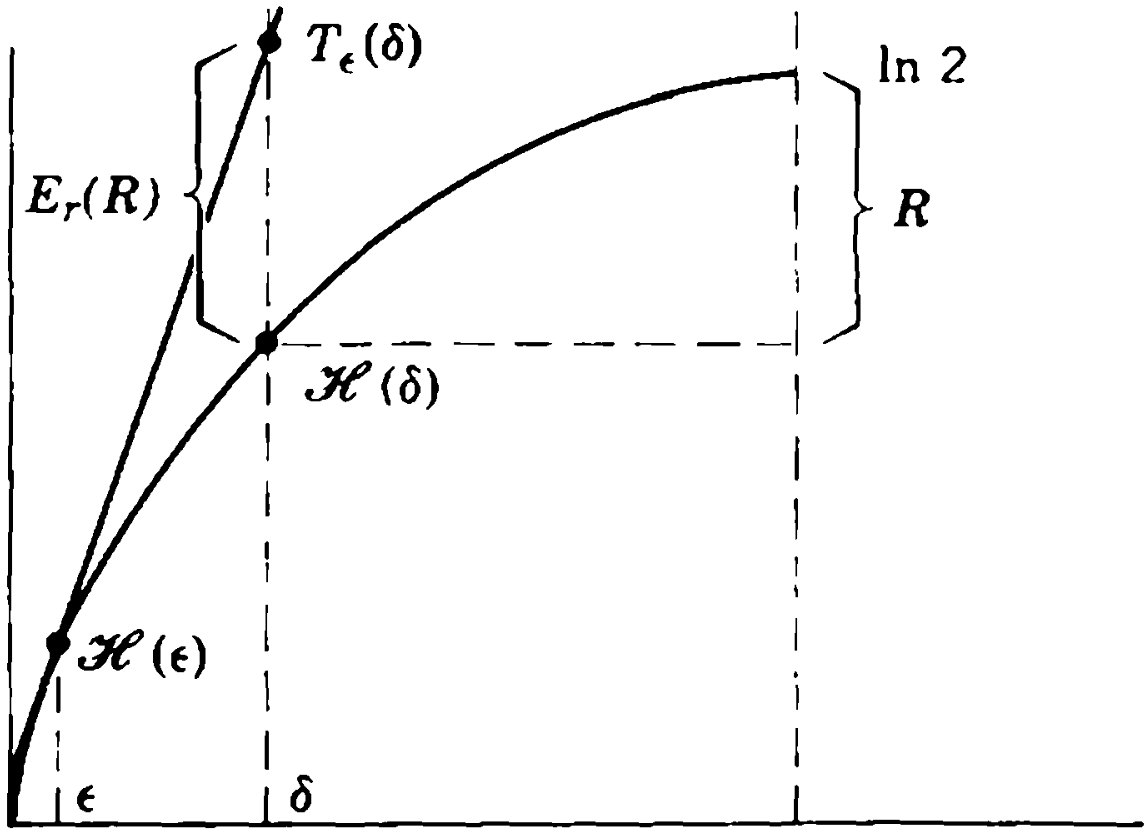
\includegraphics[scale=.25]{Fig/Entropy2.png}
    \caption{Depiction of error exponent for a binary symmetric channel, adopted from \cite{RG68}.}
    \label{Fig.Entropy2}
\end{figure}

\begin{theorem}
\label{Th.Decoding1}
Suppose that the message set for BSC consists of $M$ message and let
% ---
\begin{align}
    R = \frac{\log(M)}{N} \;,\,
\end{align}
% --
be the corresponding transmission rate in bits per channel use. If $0\leq R < C$, then there exists a coding and decoding scheme such that the error probability for each message $m$ is bounded as follows
%
\begin{align}
    P_{e,m} \leq q\cdot2^{-N\alpha(R)} \,,\,
\end{align}
%
where $q$ is a positive constant and $\alpha(R)$ is a positive function of $R$, i.e., $\alpha(R)>0$.
\end{theorem}
%%
It is important to note that the case when $1-H(\frac{\sqrt{\epsilon}}{\sqrt{\epsilon}+\sqrt{1-\epsilon}}) \leq R \leq C$, the exponent $\alpha(R) = T_{\epsilon}(\delta) - H(\delta)$ where $\delta$ is such that $H(\delta) = 1-R$ and $\epsilon < \delta \leq \frac{\sqrt{\epsilon}}{\sqrt{\epsilon}+\sqrt{1-\epsilon}}$ is our interest. In this case, the following corollary is of special interest in our next analysis.
%%
\begin{corollary}
\label{C.amount.Trans}
    Suppose the message set consists of $2^n$ messages and let $N=n(1+\frac{H(\epsilon)}{1-H(\epsilon)}+r)$, where $r$ is any arbitrarily positive small constant. Then there exists a code of length $N$ such that the worst case error probability is bounded by $q\cdot2^{-N\alpha}$ namely
    %
    \begin{align}
        \underset{m\in\{1:M\}}{\max} P_{e,m} \leq q\cdot2^{-N\alpha} \,,\,
    \end{align}
    %
    for $q=q(r,\epsilon)>0$ and $\alpha=\alpha(r,\epsilon)$.
\end{corollary}
%%%
\begin{proof}
Let $\delta > \epsilon$ be such that $H(\delta) = \frac{r + (1-r)H(\epsilon)}{r+1-rH(\epsilon)}$ (assuming $r>0$ is chosen sufficiently small such thta $\delta\leq \frac{\sqrt{\epsilon}}{\sqrt{\epsilon}+\sqrt{1-\epsilon}}$). Then $\alpha(R)$ given in Th.~\ref{Th.Decoding1} can be taken to be
%
\begin{align}
    \alpha = T_{\epsilon}(\delta) - H(\delta).
\end{align}
%
We note that the above bound can not be improved as the following theorem states.
\end{proof}
%%%%%%%%%%%%%%%%%%%%%%%%%%
\begin{theorem}[see {\cite[Th.~$5.8.5$]{RG68}}]
\label{Th.Decoding_Lowerbound}
If $R = \frac{\log(M)}{N} > C$, then the average error probability is lower bounded as follows
%
\begin{align}
    \bar{P_e} \geq 1-\frac{4A}{n(R-C)^2} - 2^{-\frac{N(R-C)}{2}}.
\end{align}
%
Where $A$ is a positive constant. Note that the above lowerbound approached 1 arbitrarily close as $N\to\infty$.
\end{theorem}
%
%%%%%%%%%%%%%%%%%%%%%%%%%%
\begin{corollary}
    If $N<n(1+\frac{H(\epsilon)}{1-H(\epsilon)})$, then there exists at least one message for which the error probability can not bounded by any constant $q<1$. This equivalently means that in order to be in the safe side and have bound for all the messages, the length $N$ of the code must satisfy
    %
    \begin{align}
        N > n(1+\frac{H(\epsilon)}{1-H(\epsilon)}) \,.\,
    \end{align}
    %
\end{corollary}
%%%
\begin{proof}
    % To prove this corollary as a result from Th.~\ref{Th.Decoding_Lowerbound} we draw the attention to the following remark from logic.
    % %
    % \begin{remark}[Contraposition]
    % \label{Rem.Contraposition}
    % From logic and law of contrapositive we have that a conditional statement if true if and only if its contraposition is true, i.e.,
    % %
    % \begin{align}
    %     A \Rightarrow B \iff B \Rightarrow A
    % \end{align}
    % %
    % in words we can state that "if A, then B" is "if not B, then not A." We note that $A$ and $B$ are both two statements which express facts about something.
    % \end{remark}
    % %
    % By Rem.~\ref{Rem.Contraposition} we can say that the Th,~\ref{Th.Decoding_Lowerbound} is logically equivalent to its contraposition which is stated as follows
    %
    To prove we just rewrite carefully what is stated in the original Th.~\ref{Th.Decoding_Lowerbound} namely
    \begin{align}
        R > C \iff \bar{P_e} \geq 1-\frac{4A}{n(R-C)^2} - 2^{-\frac{N(R-C)}{2}}  \,.\,
    \end{align}
    %
    Note that $R=\frac{\log(M)}{N}$, and $M=2^n$, hence $R>C$ is equivalent to $\frac{\log 2^n}{N} > C$ or $N<\frac{n}{C}$. Now we use the fact that $C_{BSC}=1-H(\epsilon)$, therefore we get
    %
    \begin{align}
        N&<\frac{n}{1-H(\epsilon)}\\
        &=n\cdot\frac{1}{1-H(\epsilon)}
        \\
        &=n\cdot\frac{1-H(\epsilon)+H(\epsilon)}{1-H(\epsilon)} 
        \\
        &= n\cdot(1+\frac{H(\epsilon)}{1-H(\epsilon)}) \,.\,
    \end{align}
    Hence we get the final inequality as $N<n\cdot(1+\frac{H(\epsilon)}{1-H(\epsilon)})$.
\end{proof}
%%%%%%%%%%%%%%%%%%%%%%%%%%
%\begin{corollary}
%\label{Corollary.R>C}
    %Let $\lambda$ be any arbitrarily large positive constant. Then there exists an $\epsilon\in]0,\frac{1}{2}[$, such that no code of length $N<n\lambda$ can guarantee any bound $q<1$ on the maximum (worst case) error probability.
%\end{corollary}
%%%%%%%%%%%%%%%%%%%%%%%%%%
%%%
\chapter{Standard Identification}
In this Chapter the standard identification over a Binary Symmetric channel is introduced. furthermore a Theorem will be stated and proved.
\label{Standard.Identification}
\subsubsection{System model}
\begin{figure}[!htb]
    \centering
	\scalebox{1}{
\tikzstyle{farbverlauf} = [ top color=white, bottom color=white!80!gray]
\tikzstyle{block1} = [draw,top color=white, middle color=cyan!30, rectangle, rounded corners,
minimum height=2em, minimum width=2.5em]

\tikzstyle{block2} = [draw,top color=white, middle color=cyan!30, rectangle, rounded corners,
minimum height=2em, minimum width=2.5em]

\tikzstyle{input} = [coordinate]
\tikzstyle{sum} = [draw, circle,inner sep=0pt, minimum size=5mm,  thick]
\tikzstyle{arrow}=[draw,->]

\begin{tikzpicture}[auto, node distance=2cm,>=latex']
\node[] (M) {$i$};
\node[block1,right=.5cm of M] (enc) {Enc};
\node[sum, right=3cm of enc] (channel) {$+$};

\node[below=.5mm of channel] (mod2) {$\text{\scriptsize mod 2}$};

\node[block2, right=1.5cm of channel] (dec) {Dec};
\node[below=.5cm of dec] (Target) {$j$};
\node[right=.5cm of dec] (Output) {$\text{\small Yes/No}$};

\node[above=.7cm of channel] (noise) {$\textbf{Z}\sim \text{Ber($\epsilon$)}$};
\draw[->] (M) -- (enc);
\draw[->] (enc) --node[above]{$\textbf{u}_i$} (channel);
\draw[->] (noise) -- (channel);
\draw[->] (channel) --node[above]{$\textbf{Y}$} (dec);

\draw[->] (dec) -- (Output);
\draw[->] (Target) -- (dec);

\end{tikzpicture}
}

	\caption{Deterministic message identification for the binary symmetric channel}
	\label{Fig.BSC_Channel}
\end{figure}
%%%

\begin{remark}
Assuming that $i$ enters the encoder and $\fu_{\text{i}}$ of length $N$ was selected for transmission through the channel, then number of crossovers that occur in the channel is $d_{\text{H}}(\fu_{\text{i}},\fy)$ (the output at receiver located $K$ bits away in the sense of Hamming metric from $\fu_{\text{i}}$). This implies the channel transition probability for BSC as follow
%%%
\begin{align}
    \Pr\left(\fy|\fu_{\text{i}}\right) = \epsilon^{d_{\text{H}}(\fu_{\text{i}},\fy)}(1-\epsilon)^{N-d_{\text{H}}(\fu_{\text{i}},\fy)} \, . \,
\end{align}
%%%
Furthermore, we can write the probability that $K$ crossover happens in $N$ digits can be expressed as
%%%
\begin{align}
    \label{Eq.BinomialDist}
    \Pr\left[d_{\text{H}}(\fu_{\text{i}},\fy)=K\right] = B\left(N,\epsilon\right) = \binom{N}{K} \epsilon^K (1-\epsilon)^{N-k} \, , \,
\end{align}
%%%
where $B(N,\epsilon)$ is the binomial distribution with success probability of $\epsilon$. 
\end{remark}
% ---
 The following Theorem.~\ref{theorem.IDproblem} is inspired by the theorem (\cite{J85}, see Theorem 3.1) with an extension.
 During the analysis of the theorem cited above the following mistake was encountered: 
 \begin{itemize}
     \item Assumption that $d_{\text{H}}(\fu_{\text{i}},\fu_{\text{j}})\geq \beta N$ and $d\leq \beta N$. The mistake here is using $\geq$ and $\leq$ together; Namely in Claim.1 of Theorem 3.1. JaJa assumed 
     \begin{itemize}
         \item On one hand that All the values between $0$ and $2^n-1$ can be coded with binary sequences of length $n$, subject to the Hamming distance property $d_{\text{H}}(\fu_{\text{i}},\fu_{\text{j}})\geq \beta N$.
         \item On the other hand an exhaustion method is used in which he deletes all sequences from each code word subject to the Hamming distance $d \leq \beta N$
     \end{itemize}
      This leads to a contradiction since one of the codewords $\fu_{\text{i}}$ and $\fu_{\text{j}}$ with Hamming distance $d_{\text{H}}(\fu_{\text{i}},\fu_{\text{j}})=\beta N$ will be deleted.
 \end{itemize}
In addition to the improvements brought to the main result for standard deterministic identification \cite[see Theorem 3.1]{J85} it will be derived that the BSC Capacity for DI is exactly equal to $1$.
\begin{theorem}
\label{theorem.IDproblem}
Let $\epsilon$ satisfy $0<\epsilon<\frac{1}{2}$ and let $\gamma$ be any arbitrarily small positive constant. Then there exist a code of length $N=n(1+\gamma)$ such that the identification function $f(i,j)$ can be computed with the maximum error probability $P_e$ for any input values satisfying
%
\begin{align*}
    P_e \leq c\cdot2^{-N\alpha} \, , \,
\end{align*}
%
for $\alpha = \alpha(\gamma,\epsilon,N)>0$ and $c = c(\gamma,\epsilon,N)>0$.
This BSC capacity is given by 
\begin{align}
    \label{Th.DI}
    \mathbb{C}_{\,\text{DI}} \left( \B \right) = 1 \,.\,
\end{align}
\end{theorem}
% ---
\begin{proof}[Converse Proof]
\label{Sec.Converse}
Obviously, size of the code can not exceed the space that it belongs to, i.e., $|\X|^n = 2^N$. Therefore, size of the code, $M = 2^{NR}$ is upper-bounded as below,
% ---
\begin{align}
     2^{NR} \leq \left| \X \right|^N \,,\,
\end{align}
% ---
which implies
% ---
\begin{align}
\label{upperbound.Rate}
    R & \leq \frac{1}{N} \log\left( \left| \X \right|^N \right)
    \nonumber\\
    & = \frac{N}{N} \log \left| \X \right|
    \nonumber\\
    & = \frac{N}{N} \log \left| \X \right|
    \nonumber\\
    & = \frac{N}{N} \log 2 
    \nonumber\\
    & = 1 \,.\,
\end{align}
\end{proof}
% ---------------------------------
\begin{proof}[Achievability proof]
Our notations here are the same as in \cite{J85} unless explicitly stated. Let $0<\tilde{\gamma}<\gamma$ and let $N=n(1+\tilde{\gamma})+1+\tilde{\gamma} \leq n(1+\gamma)$ for sufficiently large $n$. Let $0<\beta<\min(\epsilon,\frac{1}{3})$ be chosen such that the following holds
%
\begin{align}
    \frac{1}{1-H(\beta)} \leq 1+\tilde{\gamma} \,.\,
\end{align}
%
We note that as $\beta$ decreases, the expression $ \frac{1}{1-H(\beta)}$ converges to $1$. 
first we check the inequality for
% ---
\begin{align}
    N=n(1+\tilde{\gamma})+1+\tilde{\gamma} \leq n(1+\gamma) \,,\,
\end{align}
% ---
for sufficiently large $n$ such that $0<\tilde{\gamma}<\gamma$
\begin{align}
    n(1+\tilde{\gamma})+1+\tilde{\gamma} &\stackrel{(a)}{\leq} n(1+\gamma)\\
    (1+\tilde{\gamma})+\frac{1+\tilde{\gamma}}{n} &\stackrel{(b)}{\leq} (1+\gamma)\\
    (1+\tilde{\gamma}) &\stackrel{(c)}{\leq} (1+\gamma)\\
    \tilde{\gamma} &\stackrel{(d)}{\leq} \gamma  \,,\,
\end{align}
where $(d)$ holds since the expression $\frac{1+\tilde{\gamma}}{n}$ goes towards zero for sufficiently large n.We can reverse the inequalities from $(d)$ to $(a)$, where from $(c)$ to $(b)$ holds for the following $n$
\begin{align}
\nonumber
    \frac{1+\tilde{\gamma}}{n} &\leq (1+\gamma)-(1+\tilde{\gamma}) \\
    \nonumber
   \frac{1+\tilde{\gamma}}{\gamma-\tilde{\gamma}} &\leq n  \,.\,
\end{align}
Further we denote the Hamming distance of two distinct vectors $\fu$ and $\fu'$ by $d_{\text{H}}(\fu,\fu')$. Further we need the following lemma to show that all the input sequence $\{0,1\}^n$ can be exhausted and used as codewords. To do this, the Lem.~\ref{Lem.Exhausting}
\end{proof}
% -----------------------------------------
\begin{lemma}[see {\cite[Claim.~$1$]{J85}}]
\label{Lem.Exhausting}
All the values between $0$ and $2^n-1$ can be coded with binary sequences of length $n$, subject to the Hamming distance property, i.e.,
%%%
\begin{align}
    d_{\text{H}}(\fu_{\text{i}},\fu_{\text{j}}) > N\beta \quad \text{ for } i \neq j\;.\,
\end{align}
%%%
\end{lemma}
%%%
\begin{proof}

\begin{remark}[see  {\cite[Problem.~5.19]{RG68}}]
Let $\C$ be a code with desired minimum Hamming distance $d_{\text{min}} \in \mathbb{Z}$ and is defined as follow
% ---
\begin{align}
    d_{\text{min}} = \underset{(\text{i},\text{j}) \in M \times M}{\min} \, d(\fu_\text{i},\fu_\text{j}) \;.\,
\end{align}
% ---
Observe that since $\beta N$ can be in principle a fractional number, therefore we take the floor of it in order to make it an integer, i.e.,
% ---
\begin{align}
    d_{\text{min}} = \floor{\beta N} + 1 \;.\,
\end{align}
% ---
Choose an arbitrary codeword $\fu_0$ for $0$. Delete all sequences of distance at most one unit less or equal than the minimum Hamming distance, i.e., of distance
% ---
\begin{align}
    d & \leq d_{\text{min}} - 1
    \nonumber\\
    & = \floor{\beta N}
    \;,\,
\end{align}
% ---
from $\fu_0$. Repeat the procedure for $1,2,...$ until all the sequences are exhausted. Let $M$ be the number of codewords obtained.\newline
If one applies the Gilbert Bound (see Def.~\ref{Th.Gilbert_Bound}) with parameters $q=2$, $A(q,n) = M$, $d=d_{min}$ then we obtain 
%%%
\begin{align}
    \label{Ineq.GilbertBound}
    M \sum_{i=0}^{d_{\text{min}}-1} \binom{N}{i} \geq 2^N.
\end{align}
%%%
The $d$ for the Gilbert bound denote the minimum Hamming distance and in \cite{J85} d is defined to be $d \leq d_{min}-1$ thus we can rewrite the equation .~\eqref{Ineq.GilbertBound} like the following 
\begin{align}
\label{Eq.GB2}
    M \sum_{i=0}^{d} \binom{N}{i} \geq 2^N,
\end{align}
where $d \leq  d_{\text{min}}-1$.
\end{remark}
%%%%%
\begin{figure}[H]
    \centering
    \input{GB.tex}
    \vspace{4mm}
    \caption{Illustration of intersecting Hamming spheres in the Gilbert bound-wise exhaustion.}
    \label{fig:my_label}
\end{figure}
%%%%%
%\begin{figure}[H]
 %   \centering
 %   % \documentclass{standalone}

\tikzset{every node/.style={scale=1.4}}

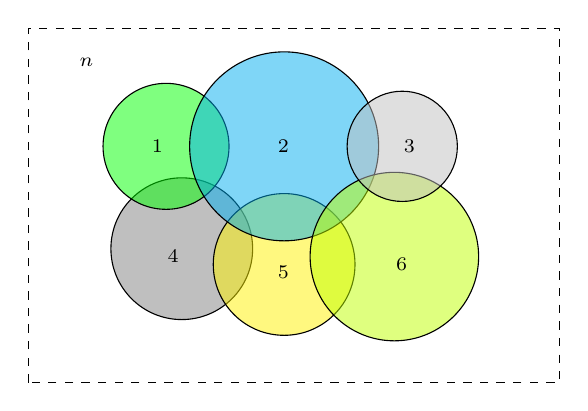
\begin{tikzpicture}
% outer dashed circle
\draw[dashed] (-0.75,1.0) rectangle (6cm, 5.5cm);

% circles 
% \draw [fill=cyan, fill opacity=0.5] (1,1) circle (1cm);
\draw [fill=gray, fill opacity=0.5] (1.2,2.7) circle (0.9cm);
\draw [fill=green, fill opacity=0.5] (1,4) circle (0.8cm);
% \draw [fill=red, fill opacity=0.5] (2.5,1) circle (1cm);
\draw [fill=yellow, fill opacity=0.5] (2.5,2.5) circle (0.9cm);
\draw [fill=cyan, fill opacity=0.5] (2.5,4) circle (1.2cm);
% \draw [fill=pink, fill opacity=0.5] (4,1) circle (1cm);
\draw [fill=lime, fill opacity=0.5] (3.9,2.6) circle (1.07cm);
\draw [fill=lightgray, fill opacity=0.5] (4,4) circle (0.7cm);


% \draw [fill=magenta, fill opacity=0.5] (1,1) circle (1cm) node {$\D_1$};
% \draw [fill=brown, fill opacity=0.5] (1,2.5) circle (1cm) node {$\D_2$};
% \draw [fill=purple, fill opacity=0.5] (2.5,1) circle (1cm) node {$\D_3$};
% \draw [fill=yellow, fill opacity=0.5] (2.5,2.5) circle (1cm) node {$\D_4$};

% labels
\node at (0.9,4) {$\D_1$};
\node at (2.5,4) {$\D_2$};
\node at (4.1,4) {$\D_3$};
\node at (1.1,2.6) {$\D_4$};
\node at (2.5,2.4) {$\D_5$};
\node at (4,2.5) {$\D_6$};
\draw (0, 5) node {$\Y^n$};

\end{tikzpicture}

    % \caption{Illustration of intersected Hamming spheres in the Gilbert bound-wise exhaustion method.}
    % \label{fig:my_label}
%\end{figure}
%%%%%
%\begin{figure}[H]
 %   \centering
  %  \scalebox{.6}{
\begin{tikzpicture}[scale=1][thick]
\draw[dashed] (0,0) circle (5cm);
\draw (0,3) circle (1.5cm);
\draw (2,1.5) circle (1.5cm);
\draw (2,-1) circle (1.5cm);
\draw (-2,2) circle (1.5cm);
\draw (-.5,.9) circle (1.5cm);
\node at (-2,0) {$\vdots$};
\node at (-.5,-1.5) {$\ldots$};
\node at (0,3) {$\D_i$};
\node at (2,1.5) {$\D_j$};
\node at (2,-1) {$\D_l$};
\node at (-2,2) {$\D_k$};
\node at (-.5,.9) {$\D_m$};
\draw[->] (0,5) -- ++(0,1)  node [fill=white,inner sep=2pt](a){$\Y^n=\X^n$};
%\draw[fill=gray] (0,0) circle (1.5cm);
\draw [fill=cyan, fill opacity=0.5, name path=i] (0,3) circle (1.5cm);
\draw [fill=orange, fill opacity=0.5, name path=j] (2,1.5) circle (1.5cm);
\draw [fill=yellow, fill opacity=0.5,name path=l] (2,-1) circle (1.5cm);
\draw [fill=gray, fill opacity=0.5, name path=k] (-2,2) circle (1.5cm);
\draw [fill=green, fill opacity=0.5, name path=k] (-.5,.9) circle (1.5cm);
\path [name intersections={of=i and j,by=cs}];
%\draw (cs) -- ++(1.5,2) node [fill=white,inner sep=2pt](c){$\propto \lambda_2^{(i,j)}$};
\draw (cs)+(-.35,-.5) -- ++(1.5,2) node [fill=white,inner sep=2pt](c){$\propto \lambda_2^{(i,j)}$};
\path [name intersections={of=l and j,by=ct}];
\draw (ct)+(-.5,0) -- ++(4,0) node [fill=white,inner sep=1pt](d){$\propto \lambda_2^{(j,l)}$};
\path [name intersections={of=i and k,by=cu}];
\draw (cu)+(.2,.2) -- ++(-3,1) node [fill=white,inner sep=5pt](e){$\propto \lambda_2^{(i,k)}$};
%\draw[dotted] (-2,-2.5) arc (-130:-160:5) ;
\end{tikzpicture}}
    % \caption{Illustration of intersected Hamming spheres in the Gilbert bound-wise exhaustion method.}
    % \label{fig:my_label}
%\end{figure}
%%%%%
The figure above  illustrates the intersection of two hamming spheres with radius $r=\floor{\beta N}$ and centers $\fu_{\text{i}}$ and $\fu_{\text{j}}$. The distance between these tow codewords is $d_{\text{min}}=\floor{\beta N}+1$. as long as $r < d_{\text{min}}$ the code size will be respected, since only the Sequences with distance $d \leq \floor{\beta N}$ will be deleted. Furthermore the intersection of the hamming spheres justifies why the Volume $V_1=  M \sum_{i=0}^{d} \binom{N}{i}$ exceed the volume space $V_2= 2^N$.\newline
Let's apply to the inequality \eqref{Lem.lemm5} with the following parameters
% ---
\begin{align}
    \epsilon&=\frac{1}{2}
    \nonumber\\
    k &= d \,,\,
\end{align}
we have then 
\begin{align}
    \label{Ineq.2option}
     \sum_{i=0}^{d} \binom{N}{i} (\frac{1}{2})^j (1-\frac{1}{2})^{(N-j)} &\leq \left[ \frac{1-\frac{d}{N}}{1-2\frac{d}{N}} \right] 2^{N\left[H(\frac{d}{N})-T_\epsilon(\frac{d}{N})\right]}
     \nonumber\\
     \sum_{i=0}^{d} \binom{N}{i} 2^{-N} &\leq \left[ \frac{1-\frac{d}{N}}{1-2\frac{d}{N}} \right] 2^{N\left[H(\frac{d}{N})-T_\epsilon(\frac{d}{N})\right]}
     \nonumber\\
     \sum_{i=0}^{d} \binom{N}{i} &\leq \left[ \frac{1-\frac{d}{N}}{1-2\frac{d}{N}} \right] 2^{N H(\frac{d}{N})} \,.\,
\end{align}
Now with the inequalities \eqref{Eq.GB2} and \eqref{Ineq.2option} we obtain 
\begin{align}
\label{ineq.2_solution}
    M \left[\frac{1-\frac{d}{N}}{1-2\frac{d}{N}} \right] 2^{N H(\frac{d}{N})} &\geq 2^N
    \nonumber\\
    M &\geq  \left[\frac{1-2\frac{d}{N}}{1-\frac{d}{N}} \right] 2^{N\left[1- H(\frac{d}{N})\right]} \,.\,
\end{align}
We have 
\begin{align}
 \frac{d}{N} &\leq \beta
 \nonumber\\
 H(\frac{d}{N}) &\leq H(\beta)
 \nonumber\\
 1 - H(\beta) &\leq 1- H(\frac{d}{N})
 \nonumber\\
  \frac{1}{1- H(\frac{d}{N})} &\leq \frac{1}{1 - H(\beta)}\,.\,
\end{align}
Note that 
% ---
\begin{align}
    \frac{1}{1-H(\beta)} &\leq 1+\widetilde{\gamma} \,,\,
\end{align}
thus 
\begin{align}
  \frac{1}{1- H(\frac{d}{N})} &\leq 1+\widetilde{\gamma} 
  \nonumber\\
  \frac{1}{1+\widetilde{\gamma}} &\leq  1- H(\frac{d}{N})
  \nonumber\\
  \frac{N}{1+\widetilde{\gamma}} &\leq  N \left[1- H(\frac{d}{N})\right]\,.\,
  \nonumber\\
\end{align}
Observe that 
\begin{align}
   \frac{N}{1+\widetilde{\gamma}}   & = \frac{n(1+\widetilde{\gamma}) + 1 + \widetilde{\gamma}}{1+\widetilde{\gamma}}
  \nonumber\\
  & = n + 1 \,,\,
\end{align}
implies 
\begin{align}
\label{ineq.2_2solution}
   n + 1  \leq  N \left[1- H(\frac{d}{N})\right]\,.\,
\end{align}
Now with the inequalities \eqref{ineq.2_2solution} and \eqref{ineq.2_solution} we conclude 
\begin{align}
\label{ineq.Solution2}
     M \geq  \left[\frac{1-2\frac{d}{N}}{1-\frac{d}{N}} \right] 2^{n+1}
\end{align}
Now focus on the term inside the bracket. Since
$\beta=\min(\frac{1}{3},\epsilon)$ where $0<\epsilon<\frac{1}{2}$, we get 
% ---
\begin{align}
    \beta &\leq \frac{1}{3}
    \nonumber\\
    \frac{d}{N} &\leq \frac{1}{3}
    \nonumber\\
    3\frac{d}{N} &\leq 1
    \nonumber\\
    4\frac{d}{N} - \frac{d}{N} &\leq 1
    \nonumber\\
    1 + 4\frac{d}{N} - \frac{d}{N} &\leq 2
    \nonumber\\
    1-\frac{d}{N}&\leq 2-4\frac{d}{N}
    \nonumber\\
    \label{Ineq.5}
    \frac{1}{2} &\leq \frac{1-2\frac{d}{N}}{1-\frac{d}{N}}\,.\,
\end{align}
Now by applying the inequalities  .~\eqref{ineq.Solution2} to .~\eqref{Ineq.5} we obtain $M\geq2^n$ and thus Lem.~\ref{Lem.Exhausting} is proved.
%--------------------------------------
Observe that $M$ is code size, it can be determined as follow
\begin{align}
    M = 2^{NR} \;,\,
\end{align}
% ---
where $R$ is the coding rate. Recall the definition as given in \eqref{Def.Rate}. Now since by \ref{Lem.Exhausting} we obtained that $M \geq 2^n$, hence, we can write $M = 2^{NR} \geq 2^n$, therefore, taking logarithm from both side yields
% ---
\begin{align}
\label{lowerbound.Rate}
    R & \geq \frac{1}{N} \log \left(2^n\right)
    \nonumber\\
    & \geq \frac{1}{(1+\gamma)n} \log \left(2^n\right)
    \nonumber\\
    & = \frac{n}{(1+\gamma)n}
    \nonumber\\
    & = \frac{1}{1+\gamma} \;.\,
\end{align}
% ---
%now since $\gamma$ can be taken any arbitrary small positive number, the lower bound for $R$ can be arbitrarily close to 1 as desired. This means that any value of $1-\delta$ for $\delta > 0$ an arbitrary constant can be achieved, that is we let
% ---
%\begin{align}
%    \frac{1}{1+\gamma} > 1 - \delta \equiv \gamma & < \frac{1}{1 - \delta} - 1
%    \nonumber\\
%    & = \frac{\delta}{1 - \delta}
%\end{align}
% ---
%To explain this more, for any arbitrarily small value $\delta$ we need only to satisfy the condition that $\gamma$ be less than $\frac{\delta}{1 - \delta}$ and then automatically (immediately) we will get
% ---
%\begin{align}
%    1 \geq R \geq 1 - \delta \;,\,
 %   \end{align}
% ---
%which means that the rate $R$ is lowerbounded by $1 - \delta$ and this is exactly the meaning of achievability. 
%To recall, the achievability notion, we should be able to find a \emph{lowerbound} for the rate in the achievability part and that lower bound here is $1-\delta$ and since $\delta$ can be made small arbitrarily as desired, thus, we infer that any value less than 1 can be a valid lowerbound for the rate, it means the rate can exceed them for or being lowerbounded by them. In other words, all values less than $1$ are achievable. This implies that capacity should be 1 if we can find a proper converse proof that 1 is upperbound for any achievable rate. We do this in a short and simple proof mention in a remark.
% -------------------
\begin{itemize}
\item  [--] Encoding: \\
Given a message $i \in [1:2^{NR}]$, transmitter sends the codeword $\fu_{\text{i}}$.
\item [--] Decoding: \\
We define the decoder as follows
% ---
\begin{align}
    \Y_{\text{j}}= \left\{ \fy \in \Y^n \;;\, d(\fy,\fu_{\text{j}}) \leq \floor{N\delta} \right\} \,.\,
\end{align}
% ---
\item [--] Error Analysis: \\
    \begin{enumerate}
        \item Type I Error: \\
        In the following section,type I error will be analyzed. The error of type I occur when $i=j$, i.e., the sent message by transmitter is exactly the one that receiver is interested in. In this case, error happens if the sequence at the output of channel, $\fy$ lies outside of the sphere with radius $\floor{N\delta}$ centered at $\fu_{\text{j}}$, where $\delta$ satisfies the following condition $\epsilon<\delta<\epsilon+ \beta(\frac{1}{2}-\epsilon)$. Therefore we have
%%%
\begin{align}
P_{e,1}(i) & = \Pr\left( \fy \in \D_{\text{i}}^c |\, \fu_{\text{i}} \right)
\nonumber\\
& = 1 - \Pr\left( \fy \in \D_{\text{i}} |\, \fu_{\text{i}} \right)
\nonumber\\
& = 1 - \Pr\left( \D_i |\, \fu_{\text{i}} \right)
% \nonumber\\
% & = 1 - \Pr\left(t \leq \ceil{N\delta} \right)
\nonumber\\
& = 1 - \Pr\left(t \leq \floor{N\delta} \right)
\nonumber\\
& = \Pr\left(t > \floor{N\delta} \right)
\nonumber\\
%& = \sum_{t=N\delta+1}^{N} \binom{N}{t} \epsilon^t (1-\epsilon)^{N-t}
%\nonumber\\
& = \sum_{t=\floor{N\delta}+1}^{N} \binom{N}{t} \epsilon^t (1-\epsilon)^{N-t} \,.\,
\end{align}
%%%
Let $k=\floor{N\delta}+1$. Observe that
% ----
\begin{align}
    \label{Ineq.Cond_3}
    \frac{k}{N} & = \frac{\floor{N\delta}+1}{N}
    \nonumber\\
    &>\frac{N\delta}{N}
    \nonumber\\
    &=\delta
    \nonumber\\
    \nonumber
    &>\epsilon \,,\,
\end{align}
% ---
thus the condition $\frac{K}{N}>\epsilon$ for the inequality \eqref{Eq.Bound2} is valid.
Now let's apply $j=t$ and $k=\floor{N\delta}+1$ to the inequality ~\eqref{Eq.Bound2} 
% ---
\begin{align}
    & \sum_{k=\floor{N\delta}+1}^{N} \binom{N}{t} \epsilon^t (1-\epsilon)^{N-t}
    \nonumber\\
    & \leq \frac{(\floor{N\delta}+1)(1-\epsilon)}{(\floor{N\delta}+1) (1-\epsilon)-[N-(\floor{N\delta}+1)]\epsilon}
    2^{-N\left[T_\epsilon\left(\frac{\floor{N\delta}+1}{N}\right)-H\left(\frac{\floor{N\delta}+1}{N}\right)\right]} \,.\,
\end{align}
% ---
Let us now focus on
% ---
\begin{align}
    \frac{(\floor{N\delta}+1)(1-\epsilon)}{(\floor{N\delta}+1) (1-\epsilon)-[N-(\floor{N\delta}+1)]\epsilon}\,.\,
\end{align}
Note that $\floor{N\delta}+1\leq N\delta+1$ then 
\begin{align}
\label{Eqfloor1}
    & \frac{(\floor{N\delta}+1)(1-\epsilon)}{(\floor{N\delta}+1) (1-\epsilon)-[N-(\floor{N\delta}+1)]\epsilon} 
    \nonumber\\
    & \leq \frac{(N\delta+1)(1-\epsilon)}{(\floor{N\delta}+1) (1-\epsilon)-[N-(\floor{N\delta}+1)]\epsilon}
    \nonumber\\
    & \leq \frac{(N\delta+1)(1-\epsilon)}{(\floor{N\delta}+1) - N\epsilon}\,.\,
\end{align}
%%%%%
Now note that 
\begin{align}
\label{Eqfloor}
    N\delta &< \floor{N\delta}+1
    \nonumber\\
    N\delta - N\epsilon &< \floor{N\delta}+1 -N\epsilon
    \nonumber\\
   \frac{1}{N\delta - N\epsilon} &> \frac{1}{\floor{N\delta}+1 -N\epsilon}\,.\,
\end{align}
%%%%%%
With the inequalities \eqref{Eqfloor} and \eqref{Eqfloor1} we obtain 
\begin{align}
\label{upperboundtype1}
\frac{(\floor{N\delta}+1)(1-\epsilon)}{(\floor{N\delta}+1) (1-\epsilon)-[N-(\floor{N\delta}+1)]\epsilon} & \leq \frac{(N\delta+1)(1-\epsilon)}{N\delta - N\epsilon}
\nonumber\\
\frac{(\floor{N\delta}+1)(1-\epsilon)}{(\floor{N\delta}+1) (1-\epsilon)-[N-(\floor{N\delta}+1)]\epsilon} & \leq \frac{\left(\delta+\frac{1}{N}\right)\frac{(1-\epsilon)}{N}}{\delta - \epsilon}\,.\,
\end{align}
%%%%
Now with the inequalities \eqref{upperboundtype1} and \eqref{Eqfloor1} we obtain 
\begin{align}
\label{Eq-typeI}
 \sum_{k=\floor{N\delta}+1}^{N} \binom{N}{t} \epsilon^t (1-\epsilon)^{N-t} \leq \frac{\left(\delta+\frac{1}{N}\right)\frac{(1-\epsilon)}{N}}{\delta - \epsilon} 2^{-N\left[T_\epsilon\left(\frac{\floor{N\delta}+1}{N}\right)-H\left(\frac{\floor{N\delta}+1}{N}\right)\right]} \,.\,
\end{align}
Since  $T_\epsilon(\frac{\floor{N\delta}+1}{N})-H(\frac{\floor{N\delta}+1}{N})>0$ and $\delta > \epsilon$ the upper bound goes towards zero as N goes towards infinity. Thus the proof for type I error is complete.
% ----------------
        \item Type II Error: \\
        The error of type II occur when $i\neq j$. In this case, error happens if the sequence at the output of channel, $\fy$ lies 
        \begin{itemize}
            \item Inside the intersection of spheres with radius $\floor{N\delta}$ centered at $\fu_{\text{j}}$ and the sphere with radius $\floor{N\delta}$ centered at $\fu_{\text{i}}$
            \item Outside of the sphere $\floor{N\delta}$ centered at $\fu_{\text{i}}$ centered at with $\fu_{\text{i}}$ and inside the sphere $\floor{N\delta}$ centered at $\fu_{\text{j}}$ centered at with $\fu_{\text{j}}$
        \end{itemize}  
% ---
then we have
% ---
\begin{align}
   P_{e,2}(i,j) &= \sum_{\Y_{\text{j}}} p(\fy|\fu_{\text{i}})
   \nonumber
   \\
   \label{Eq.TypeIIError}
   &= \sum_{\Y_{\text{j}} \; \cap \; \Y_{\text{i}}} p(\fy \given \fu_{\text{i}}) +  \sum_{\Y_{\text{j}} \; \cap \; \Y_{\text{i}}^c} p(\fy \given \fu_{\text{i}})
   \nonumber
   \\
  &= \sum_{d_{\text{H}}(\fy,\fu_{\text{j}}) \leq \floor{N\delta} \;\cap \; d_{\text{H}}(\fy,\fu_{\text{i}}) \leq N\delta} p(\fy \given \fu_{\text{i}}) 
  \nonumber\\
  & + \sum_{d_{\text{H}}(\fy,\fu_{\text{j}}) \leq \floor{N\delta} \;\cap \; d_{\text{H}}(\fy,\fu_{\text{i}}) > N\delta} p(\fy \given \fu_{\text{i}})
  \nonumber
   \\
    &= S_1+S_2\,.\,
\end{align}
%%%
In the second sum in equation \eqref{Eq.TypeIIError} the output of channel, $\fy$ lies outside of the decoding region with center $\fu_{\text{i}}$ and inside the decoding set with center $\fu_{\text{j}}$. therefor it wouldn't be in the intersection of the regions that this condition specifies. \newline The law of total probability implies the following inequality for these two events:
% ---
\begin{align}
    \label{event.Ineq}
    \left|\left(d_{\text{H}}(\fy,\fu_{\text{j}}) \leq \floor{N\delta}\right) \;\cap \; \left(d_{\text{H}}(\fy,\fu_{\text{i}}\right) > N\delta)\right|  < \left|d_{\text{H}}(\fy,\fu_{\text{i}}) \leq \floor{N\delta} \right| \,.\,
\end{align}
% ---
Hence
\begin{align}
    & \sum_{\fy\;;\,d_{\text{H}}(\fy,\fu_{\text{j}}) \leq \floor{N\delta} \; \cap \; d_{\text{H}}(\fy,\fu_{\text{i}}) > N\delta} p(\fy|\fu_{\text{i}})
    \nonumber\\
    & < \sum_{\fy\,:\, d_{\text{H}}(\fy,\fu_{\text{i}})  > N\delta} p(\fy|\fu_{\text{i}}) 
    \nonumber\\
    & \leq \frac{\left(\delta+\frac{1}{N}\right)\frac{\left(1 - \epsilon\right)}{N}}{\delta - \epsilon} 2^{-N\left[T_\epsilon\left(\frac{\floor{N\delta}+1}{N}\right)-H\left(\frac{\floor{N\delta}+1}{N}\right)\right]}
    \,,\,
\end{align} 
%%%
where the last inequality is due to the equation \eqref{Eq-typeI}.\newline
To address the first sum in the equation \eqref{Eq.TypeIIError} let $d_{\text{H}}=d_{\text{H}}(\fu_{\text{i}},\fu_{\text{j}}) > \beta N$. This means that $\fu_{\text{i}}$ and $\fu_{\text{j}}$ differ in $d_{\text{H}}$ bits. Without loss of generality we assume that
%%%
\begin{align}
    \label{Eq.Sequences}
    &\fu_\text{i} = (u_{\text{i}_1},u_{\text{i}_2},\ldots,u_{\text{i}_\text{d}},u_{\text{i}_\text{d+1}},\ldots,u_{\text{i}_\text{n}})\,,\,
    \nonumber
    \\
    &\fu_\text{j}= (u_{\text{j}_1},u_{\text{j}_2},\ldots,u_{\text{j}_\text{d}},u_{\text{i}_\text{d+1}},\ldots,u_{\text{i}_\text{n}})\,,\,
    \nonumber
    \\
    &\fy = (y_1,y_2,\ldots,y_\text{d},y_\text{d+1},\ldots,y_\text{n})\,.\,
 \end{align}
%%%
That is, the two $N$-sequence $\fu_{\text{i}}$ and $\fu_{\text{j}}$ differs only in their first $d$ bits and share rest of the $N-d$ bits in common. Now the event $d_{\text{H}}(\fy,\fu_{\text{i}}) \leq \floor{N\delta}$ implies that the received vector $\fy$ disagree with $p$ bits of $\fu_{\text{i}}$, when $p\leq \floor{N\delta}$, i.e.,
%%%
\begin{align}
    d_{\text{H}}(\fy,\fu_{\text{i}}) = p \leq \floor{N\delta} \,.\,
\end{align}
%%%
Further, we assume on one hand that $p_1\leq p$ bits among $p$ bits are located in $u_{\text{i}_1},u_{\text{i}_2},\ldots,u_{\text{i}_{\text{d}}}$, i.e. $d_H(\fy|_1^d,{\fu_\text{i}}|_1^d) = p_1$ , and on the other hand $p_2=p-p_1$ are among $u_{\text{i}_{d+1}},\ldots,u_{\text{i}_{\text{n}}}$, i.e. $d_H(\fy|_{d+1}^N,{\fu_\text{i}}|_{d+1}^N) = p_2$ .\newline 
First we focus on the RHS tail, i,e,
%
\begin{align}
 \fy|_{d+1}^N \text{ versus } {\fu_\text{i}}|_{d+1}^N\,.\,
\end{align}
%
Since ${\fu_\text{i}}|_{d+1}^N = {\fu_\text{j}}|_{d+1}^N$,
it implies that $y_{d+1},\ldots,y_N$ also differs in exactly $p_2$ bits with tail of $\fu_\text{j}$, i.e.
%%%
\begin{align}
    d_{\text{H}}\left(\fy|_{d+1}^N,{\fu_\text{j}}|_{d+1}^N\right) = p_2\,.\,
\end{align}
%%%
Now we focus on the LHS tail
%
\begin{align}
 \fy|_1^{d} \text{ versus } {\fu_\text{i}}|_1^{d}\,.\,
\end{align}
%
Note that $\fu_\text{i}$, $\fu_\text{j}$ and $y$ are binary alphabet, i.e there is only two possible values for each bit namely \{0,1\}. $d=d_{\text{H}}(\fu_\text{i},\fu_\text{j})$ implies for the case of binary alphabets that ${\fu_\text{i}}|_1^{d}$ and ${\fu_\text{j}}|_1^{d}$ are complementary for the first $d$ bits. Now this is relevant to determinate in how many bits ${\fu_\text{j}}|_1^{d}$ and  ${\fy}|_1^{d}$ differ knowing that $d_{\text{H}}(\fy|_1^d,{\fu_\text{i}}|_1^d) = p_1$. If $p_1$ bits are different for $\fy|_1^d$ and $\fu_\text{i}|_1^d$, $p_1$ bits are identical for $\fy|_1^d$ and $\fu_\text{j}|_1^d$. Thus we obtain
%%%
\begin{align}
    d_{\text{H}}(\fy|_1^d,{\fu_\text{j}}|_1^d) = d-p_1\,.\,
\end{align}
%%%
Now if we collect all possible candidate of location that the two sequence $\fy$ and $\fu_\text{j}$ can be different are exactly the sum of candidates in the two tails, i.e,
%%%
\begin{align}
    d_{\text{H}}(\fy|_1^N,{\fu_\text{j}}|_1^N) = d_{\text{H}}(\fy|_1^d,{\fu_\text{j}}|_1^d)+d_H(\fy|_{d+1}^N,{\fu_\text{j}}|_{d+1}^N)= d-p_1+p_2\,.\,
\end{align} 
%%%
Note that  $d_{\text{H}}(\fy,\fu_\text{j})\leq \floor{N\delta}$. Hence
%%%
\begin{align}
    d_{\text{H}}(\fy|_1^N,{\fu_\text{j}}|_1^N) &\leq \floor{N\delta}
    \\
    \Rightarrow d-p_1+p_2 &\leq \floor{N\delta}
    \\
    \Rightarrow p_2 &\leq \floor{N\delta}-d+p_1.
\end{align} 
On the other hand note that $d_{\text{H}}(\fy,\fu_\text{j})\leq \floor{N\delta}$. Hence 
\begin{align}
    p &\leq\floor{N\delta}
    \\
    \Rightarrow p_1+p_2 &\leq \floor{N\delta}
    \\
    \Rightarrow p_2 &\leq \floor{N\delta}-p_1.
\end{align} 
%%%%%%%%%%%%%%%%%%%%%%%%%%%%%%%%%%%%%%%
The term $S_1$ can be calculated by fixing $p_1$ and then summing over all possible cases of $p_2$. i.e. for each value of $p_1$ over d bits we sum all possible value that $p_2$ can take over $\min\{\floor{N\delta}-p_1,\floor{N\delta}-d+p_1\}$ bits. Since each of those cases are independent, therefore, the union becomes a sum. Note that the error probability is binomial distributed as mentioned in equation \eqref{Eq.BinomialDist}.
% ---
\begin{align}
    \label{S1.ineq}
    S_1 &\leq \sum_{p_1=0}^d \binom{d}{p_1} \sum_{p_2=0}^{\min\left\{\floor{N\delta}-p_1,\floor{N\delta}-d+p_1\right\}} \binom{N-d}{p_2} \epsilon^{p_1+p_2} (1-\epsilon)^{N-\left(p_1+p_2\right)+d-d}
    \nonumber\\
    & = \textcolor{black}{\sum_{p_1=0}^d \binom{d}{p_1} \epsilon^{p_1} (1-\epsilon)^{d-p_1}} 
    \nonumber\\
    & ~ \times \textcolor{black}{\sum_{p_2=0}^{\min\left\{\floor{N\delta}-p_1,\floor{N\delta}-d+p_1\right\}} \binom{N-d}{p_2} \epsilon^{p_2} (1-\epsilon)^{N-d-p_2}}\,.\,
\end{align}
%
Note that every expression that is independent of the sum variables can be  shifted left behind the sum. In order to obtain the correct form for two binomial distribution expressions, $+d-d$ is needed in \eqref{S1.ineq}. Now easily we can see that by axiom of probability [\cite{Ross14}, see P.~27] the first expression we have
%
\begin{align}
    \textcolor{black}{\sum_{p_1=0}^d \binom{d}{p_1} \epsilon^{p_1} (1-\epsilon)^{d-p_1}} = \Pr (p_1\leq d) = 1\,.\,
\end{align}
%
For the second expression, let's first set $p_1= \floor{\frac{d}{2}}$ thus 
\begin{align}
    \min\left\{\floor{N\delta}-\floor{\frac{d}{2}},\floor{N\delta}-d+\floor{\frac{d}{2}}\right\} = \floor{N\delta}-d+\floor{\frac{d}{2}}\,.\,
\end{align}
Since $\floor{\frac{d}{2}} \leq \frac{d}{2}$ implies $\frac{d}{2}\leq d-\floor{\frac{d}{2}}$.\newline
Now let's apply 
$K=\floor{N\delta}-d+\floor{\frac{d}{2}}$, $j=p_2$ , $N=N-d$ and $\frac{K}{N}=\frac{\floor{N\delta}-d+\floor{\frac{d}{2}}}{N-d}\overset{\text{def}}{=}\tau_N $ to the Inequality \eqref{Lem.lemm5}. We obtain 
%%
\begin{align}
       \label{Ineq.p_2}
        \sum_{p_2=0}^{\floor{N\delta}-d+\floor{\frac{d}{2}}} \binom{N-d}{p_2}\epsilon^{p_2} \left(1-\epsilon\right)^{N-d-p_2} & \leq \frac{\epsilon-\tau_N \cdot\epsilon}{\epsilon - \tau_N} \cdot 2^{N\left[H(\tau_N)-T_{\epsilon}(\tau_N)\right]}\,.\,
    \end{align}
%%    
Note that by the Hamming distance property we have $d=d_{\text{H}}(\fu_\text{i},\fu_\text{j}) > \beta N$ and the restriction on the threshold value of the decoder we have $\delta \leq \epsilon+\beta(\frac{1}{2}-\epsilon)$. Hence 
% ---
\begin{align}
\label{Ineq2}
 \frac{\floor{N\delta}-d+\floor{\frac{d}{2}}}{N-d} & \leq \frac{N\delta-d+\frac{d}{2}}{N-d}
 \nonumber\\
 & = \frac{N\delta-\frac{d}{2}}{N-d}
 \nonumber\\
 & \stackrel{(a)}{\leq} \frac{N\delta-\frac{\beta N}{2}}{N-\beta N}
 \nonumber\\
 & \leq \frac{\delta-\frac{\beta }{2}}{1-\beta}
 \nonumber\\
 & \overset{\text{def}}{=} \tau
%  \nonumber\\
%   \tau_N &\leq \tau
  \,,\,
\end{align}
% ---
where $(a)$ holds since $d > \beta N$.
In order for the upper bound to be positive the condition $\tau < \epsilon$ must be valid. Observe that 
\begin{align}
    \delta &< \epsilon+\beta(\frac{1}{2}-\epsilon)\,,\,
    \nonumber
\end{align}
% ---
implies
\begin{align}
\label{Ineq1}
   \delta &< \epsilon+\frac{\beta}{2} -\beta \epsilon
   \nonumber\\
   \delta - \frac{\beta}{2} &< \epsilon -\beta \epsilon
   \nonumber\\
     \delta - \frac{\beta}{2} &< \epsilon (1 -\beta)
    \nonumber\\
     \frac{\delta - \frac{\beta}{2}}{(1 -\beta)}&< \epsilon 
      \nonumber\\
     \tau &< \epsilon  < \frac{1}{2}\,.\,
\end{align}
the inequalities \eqref{Ineq2} and \eqref{Ineq1} implies that 
\begin{align}
    \tau_N < \epsilon < \frac{1}{2}\,.\,
\end{align}
Now with inequalities \eqref{Ineq2} and \eqref{Ineq.p_2} 
%%
 \begin{align}
 \label{prooftype2}
 \sum_{p_2=0}^{\delta N -d+\floor{\frac{d}{2}}} \binom{N-d}{p_2}\epsilon^{p_2}  (1-\epsilon)^{N-d-p_2} &\leq \frac{\epsilon(1-\tau)}{\epsilon-\tau}\cdot 2^{-N\left[T_{\epsilon}(\tau_N) - H(\tau_N)\right]}\,.\,
\end{align}
%
Now since $\tau < \epsilon$ and the exponent $\alpha(R) = T_{\epsilon}(\tau_N) - H(\tau_N)$ is positive the upper-bound goes to zero for sufficiently large $N$. Thus the proof for type II error is completed.
    \end{enumerate}
\end{itemize}
% -----------------------------------------
Now recalling the achievable rate definition given in \ref{Def.Ach_Rate} together with the previous results of the achievability proof and error analysis we conclude that the Rate
\begin{align}
  \frac{1}{1+\gamma}\stackrel{(a)}{\leq} R \stackrel{(b)}{\leq} 1  \,,\,
\end{align}
where (a) holds from the inequality \eqref{lowerbound.Rate} and (b) from the inequality \eqref{upperbound.Rate}, is achievable. Note that $\gamma>0$ is a positive small constant that can be arbitrarily taken to be close to zero. This implies that the term $\frac{1}{1+\gamma}$ is arbitrary close to $1$ if $\gamma$ is arbitrarily close to zero. \newline
%Thus 
%\begin{align}
%     \frac{1}{1+\gamma}\leq R \leq 1 \implies 1-\tau\leq R \leq 1 \,,\,
%\end{align}
%when $\tau$ is constant arbitrarily close to zero.
Now with the capacity begin the supremum of the achievable rate we have 
\begin{align}
 \mathbb{C}_{\text{DI}}\left( \B \right) &= \sup R \\
 & = 1 \,.\,
\end{align}
Thus the proof for the Theorem.\ref{theorem.IDproblem} is complete.\newline
%
Another way to conclude that the BSC Capacity is equal to $1$ From the definition.\ref{Def.Ach_Rate} we have 
\begin{align}
    \label{Ineq.Achiev_Rate}
    \frac{\log{M}}{N} > R - \delta  \,.\,
\end{align}
% ---
Observe that this is equivalent to
\begin{align}
    M > 2^{N(R-\delta)} \,.\,
\end{align}
% ---
In order to show that any rate arbitrarily close to $1$ is achievable, we should be able to
show that any $R$ of form $1-\tau$ where $\tau > 0$ is an arbitrary constant, can be substituted in the (\ref{Ineq.Achiev_Rate}), i.e., we should have
% ---
\begin{align}
    M & > 2^{N(1-\tau-\delta)}
    \nonumber\\
    & = 2^{N(1-(\tau+\delta))}
    \,.\,
\end{align}
% ---
Observe that we already know from result of Claim~1 that $M$ is lower bounded by $2^n$, i.e.,
% ---
\begin{align}
    \label{Ineq.Claim_1_Result}
    M & \geq 2^n \,.\,
\end{align}
% ---
Now observe that by the assumption given in the statement of Theorem~\ref{theorem.IDproblem} $N \leq n(1+\gamma)$, hence, a lower bound for the $n$ can be stated as
% ---
\begin{align}
    n \geq \frac{N}{1+\gamma} \,.\,
\end{align}
% ---
Therefore by (\ref{Ineq.Claim_1_Result}), we obtain
\begin{align}
    M \geq 2^{\frac{N}{1+\gamma}}
    \,,\,
\end{align}
% ---
Now motivating by $a\geq b$ and $b\geq c$ gives $a\geq c$, one can argue that if
we show
% ---
\begin{align}
    \label{Ineq.b>c}
    2^{\frac{N}{1+\gamma}} \geq 2^{N(1-(\tau+\delta))} \,,\,
\end{align}
% ---
then automatically we would get
% ---
\begin{align}
    M \geq 2^{N(1-(\tau+\delta))} \,,\,
\end{align}
% ---
and we will be immediately finished with the fact that $1-\tau$ is achievable.
Now we focus to show Ineq.~(\ref{Ineq.b>c}) as follows
% ---
\begin{align}
    2^{\frac{N}{1+\gamma}} \geq 2^{N(1-(\tau+\delta))} \,,\,
\end{align}
% ---
which is equivalent to show
% ---
\begin{align}
    \frac{N}{1+\gamma} \geq N(1-(\tau+\delta)) \,,\,
\end{align}
% ---
and itself is equivalent to
% ---
\begin{align}
    \frac{1}{1+\gamma} \geq 1-(\tau+\delta) \,,\,
\end{align}
% ---
or
% ---
\begin{align}
    1+\gamma \leq \frac{1}{1-(\tau+\delta)} \,,\,
\end{align}
% ---
which means that
% ---
\begin{align}
    \label{Ineq.gamma}
    \gamma \leq \frac{1}{1-(\tau+\delta)} - 1 \,,\,
\end{align}
% ---
and this condition on the $\gamma$ cab be easily fulfilled for any value of $\tau$ and $\delta$. In other word, as long as $0 < \tau + \delta < 1$, then no matter what the exact value of $\tau$ and $\delta$ are, we can always make the $\gamma$ small enough such that its value is upper bounded by $\frac{1}{1-(\tau+\delta)} - 1$. Thus, since we are able to fulfill the condition given in (\ref{Ineq.gamma}), it means that we had shown that $1-\tau$ is achievable.

Now, in order to derive a supremum for these achievable rates of the form $1-\tau$, we first derive an upper bound for the rate $R$. This upper bound is $1$ and its proof is given in Th.\ref{Sec.Converse}. Therefore any upper bound on the rate $R$ is valid also for the achievable rates. Thus, for an achievable rate $R$ we have
% ---
\begin{align}
    1 - \tau = R \leq 1 \,,\,
\end{align}
% ---
and the supremum of such achievable rate, $R$ is obviously the unique value $1$. This completes the proof that deterministic identification capacity of BSC is $1$, that is,
% ---
\begin{align}
    \mathbb{C}_{\,\text{DI}} \left( \B \right) = 1 \,.\,
\end{align}
% ---
This completes the proof of Theorem.~\ref{theorem.IDproblem}.
\end{proof}
% ---
%%%%%%%%%%%%%
\subsection{Penalty factor}
In this section we will examine a new parameter called the penalty factor, which provides valuable insight into how far the minimum required amount of communication for a reliable transmission/identification deviates from communication through perfect channel.  
\begin{definition}[\cite{J85},see P.~48]
Let $I_\epsilon(n)$ be the minimum amount of communication required to solve a given problem such that the probability of error goes to 0 as n grows large, with $\epsilon$ being the crossover probability of the channel. The penalty factor is defined to be
\begin{align}
\label{penalty.factor}
    \delta(\epsilon)= \sup_{n} \left[ \frac{I_\epsilon(n)}{I_0(n)} \right] \,,\,
\end{align}
where $I_0(n)=n$.
\end{definition}
In order to compare the penalty factor for transmission and Identification, let's first determine the minimum amount of communication for each case that is required to solve a given problem such that the error probability goes to 0 as n grows large. For the transmission as shown in Corollary.~\ref{C.amount.Trans} the minimum amount of communication for a reliable transmission is 
\begin{align}
\label{Min.Trans}
    N=(\frac{1}{1-H(\epsilon)}+r)\cdot n \, ,\,
\end{align}
where $r$ is any arbitrarily positive small constant.
Now with the equations \eqref{Min.Trans} and \eqref{penalty.factor} we obtain 
\begin{align}
    \delta(\epsilon)&= \sup_{n} \frac{(\frac{1}{1-H(\epsilon)}+r)\cdot n}{n}
      \nonumber\\ &=\sup_{n}\frac{1}{1-H(\epsilon)}+r
    \nonumber\\
    &=\frac{1}{1-H(\epsilon)}+r
\end{align}
% ---
\begin{align}
    \delta(\epsilon) & = \sup_{n} \left[ \frac{\left( \frac{1}{1-H(\epsilon)} + r \right) \cdot n}{n} \right]
    \nonumber\\
    & = \sup_{n} \left[ \frac{\left( \frac{1}{1-H(\epsilon)} \right) \cdot n}{n} + \frac{rn}{n}\right]
    \nonumber\\
    & \leq \sup_{n} \left[ \frac{\left( \frac{1}{1-H(\epsilon)} \right) \cdot n}{n} \right] + \sup_n \left[ \frac{rn}{n} \right]
    \nonumber\\
    & = \sup_{n} \left[ \frac{1}{1-H(\epsilon)} \right] + \sup_n \left[ r \right]
    \nonumber\\
    & = \frac{1}{1-H(\epsilon)} + r
\end{align}
% ---
this implies 
\begin{align}
    \delta(\epsilon) \geq \frac{1}{1-H(\epsilon)}\, .\,
\end{align}
For the identification case the following corollary is of major interest. 
\begin{corollary}
Let $\epsilon$ satisfy $0 < \epsilon <\frac{1}{2}$. The identification problem can be solved with $n + o(n)$ bits of one-way communication such that, for any pair of input values, the probability of error goes to $0$ as $n$ grows large.
\end{corollary}
\begin{proof}
By theorem.~\ref{theorem.IDproblem}, it follows that for all $\gamma,\delta>0$, there exists $n_0 =n_0(\gamma,\delta)$ such that for $n\geq n_0$ the identification problem can be solved with a code of length $\leq (1+\gamma)n$ and probability of error $\leq \delta$.
Consider the sequence of integers $n_0(\frac{1}{r},\frac{1}{r})$, $r =
1,2,3,...$, which can be assumed to be increasing. For % ---
\begin{align}
    n_0(\frac{1}{r},\frac{1}{r}) \leq n < n_0(\frac{1}{r+1},\frac{1}{r+1})
\end{align}
% ---
use the scheme that gives a code of length $\leq (1 + \frac{1}{r})n$
and probability of error $\leq \delta$. 
\begin{definition}
[\cite{hardy79}, see P.~7-8]
\label{oNotation}
let $\phi(n)$ be a positive function and $f(n)$ any function. then $f(n)=o(\phi(n))$ if the following condition is valid
% ---
\begin{align}
    \lim_{n \to \infty} \frac{f(n)}{\phi(n)} = 0 \,,\,
\end{align}
% ---
\end{definition}
It is clear that the corresponding code will be of length $n + o(n)$, and the probability of error goes to $0$ as $n$ goes to infinity.
\end{proof}
the code length for Identification can be bounded as follow:
\begin{align}
    n< N \leq (1+\gamma)n
\end{align}
Now since $n<N$, $N$ can be taken to be $N=\kappa+n$ as long as the follwing condition for $\kappa$ is valid
\begin{align}
    \kappa+n \leq (1+\gamma)n
    \nonumber\\
    \kappa \leq \gamma n
\end{align}
Now by Def.~\ref{oNotation} let's check if we can write $\kappa=o(n)$
\begin{align}
\kappa &\leq \gamma n
\nonumber\\
\lim_{n \to \infty}  \frac{\kappa}{n} &\leq %\lim_{n \to \infty} \frac{\gamma n}{n}
\nonumber\\
\lim_{n \to \infty}  \frac{\kappa}{n} &\leq \gamma
\end{align}
% \textcolor{blue}{$\frac{\kappa}{n} \leq \gamma$ and not $\frac{\kappa}{n} < \gamma$ so we technically if it's not strictly less $\kappa<\gamma n$ we cannot take it to be 0 as it can be equal to $\gamma>0$ }.\newline
Now observe that for the identification we have
% ---
\begin{align}
    \delta(\epsilon) & = \sup_n \left[ \frac{I_{\epsilon}(n)}{I_0(n)} \right]
    \nonumber\\
    & = \sup_n \left[ \frac{n + o(n)}{n} \right]
    \nonumber\\
    & = \sup_n \left[ 1 + \frac{o(n)}{n} \right]
    \nonumber\\
    & = 1 + \sup_n \left[ \frac{o(n)}{n} \right]
    \nonumber\\
    & = 1 \,,\,
\end{align}
% ---
where the last line holds via following argument: at Observe that by definition of small o notation we have that if $f(n) = o(g(n))$ then $\forall k > 0$ we have $\frac{f(n)}{g(n)} < k$ as $n \to \infty$. Thereby, $\frac{o(n)}{n}$ means that for a $f(n) = o(n)$ and $g(n) = n$ we have $\forall k > 0$ $\frac{f(n)}{g(n)} < k$ as $n \to \infty$. Now since if $a < b$ then $\sup(a) < \sup(b)$ we obtain $\sup \frac{f(n)}{g(n)} < \frac{f(n)}{g(n)} < k$. Hence, since $k$ can be arbitrarily small close to zero the value of $\sup \frac{f(n)}{g(n)}$ must exactly coincide zero, i.e., $\sup \frac{f(n)}{g(n)} = 0$.
% ---------------------------------
\chapter{K-Identification}
\label{K-ID-Chapter}
Throughout this section, we will introduce the K-Identification, which is an extension of the standard identification, in the sense that instead of having only one message at the receiver, we have $K$ many messages. \cite{Ahlswede08,Yamamoto14}. The identification problem introduced by Ahlswede and Dueck in 1989 \cite{AD89,Ahlswede21_Book} involves a decoder with only one target message, i.e. the receiver is interested to know whether that only one target message was sent or not. In the $K$-identification, the receiver is able to expand its interest by enlarging the number of target messages. The goal here is to check weather or not the sent message belongs to the set of target messages.
Our system model consist of $\Pi_{\text{k}} = \left\{ \pi_{\text{s}}:\lvert \mathcal{S} \lvert=\mathcal{K}, \mathcal{S}\subset \mathcal{M} \right\}$ with $\pi_{\text{s}}=\left\{ \mathcal{S}, \mathcal{M} \setminus \mathcal{S} \right\}$
% ------------------------------------------------
\begin{definition}
%[\cite{Ahlswede08}, see P.~1352]
an $(n, N, K,\lambda)$-code is a family of pairs
% ---
\begin{align}
    \left\{(u_{\text{i}},D_\pi):1 < i < N ,\pi \in \Pi_{\text{k}} \right\} \,,\,    
\end{align}
% ---
where $i\in \mathcal{X}^ n$, $D_\pi \subset \mathcal{Y}^ n$ and where for all partition $\pi$ such that
% ---
\begin{align}
    \pi=\left\{\mathcal{S},\mathcal{M} \setminus \mathcal{S}\right\} \left( \mathcal{S}\in \binom{\mathcal{K}}{\mathcal{M}} \right) \,.\,
\end{align}
% ---
% ---
The errors are defined as follow 
\begin{align}
    P_{e,1}(i) = W(\D_\pi^c|\fu_{\text{i}}) = \Pr(\fy\in\D_\pi^c|\fu_{\text{i}}) \leq \lambda \qquad \text{     , for all $i\in \mathcal{S}$ } \\
    \label{type2.k}
     P_{e,2}(i) = W(\D_\pi|\fu_{\text{i}}) = \Pr(\fy\in\D_\pi|\fu_{\text{i}}) \leq \lambda \qquad \text{    , for all $i\notin \mathcal{S}$ }
\end{align}
% ---
\end{definition}
% ---

\begin{theorem}
\label{Th.DKI}
Let $\B$ be a BSC with crossover probability of $0<\epsilon<\frac{1}{2}$. Then the deterministic $K$-identification capacity of a such channel is given by
% ---
\begin{align}
    \mathbb{C}_{\,\text{KDI}} \left( \B \right) = 1 \,.\,
\end{align}
% ---
\end{theorem}
% ---
\begin{proof}[Achievability Proof]
\label{Proof.Ach}
In this subsection we focus to show that an appropriate code with desired structure exist for the deterministic identification.The proof is largely  inspired by the \emph{Gilbert Bound} bound and exhaustion method that was described in the code construction of the standard identification.
Also for the K-Identification we are able to code all 
values between $0$ and $2^N-1$ with binary sequences of length $N$, subject to the Hamming distance property, i.e.,
%%%
\begin{align}
   d_{\text{H}}(\fu_{\text{i}},\fu_{\text{j}}) > N\beta \quad \text{ for } i \neq j\;,\,
\end{align}
since the difference between the standard identification and the $K$-identification starts at the decoding process. From here we can derive the upper bound for the rate that is similar to the standard identification in \eqref{lowerbound.Rate} namely 
\begin{align}
    \frac{1}{1+\gamma} \leq R \,.\,
\end{align}
% ---
\begin{itemize}
    \item [--] Encoding: \\
    Given a message $i \in [1:2^{NR}]$, transmitter sends the codeword $\fu_\text{i}$.
    \item [--] Decoding:\\
    To define a proper decoding, we need to capture the influence of having multiple target messages at hand, therefore a naive and simple idea that works is to incorporate them all by taking the union of all them. That is, the decoding set for $K$-identification as follows
    % ---
    \begin{align}
        \label{Def.Dec_KDI}
        D_{\pi} & = \bigcup_{\text{j} \in \S} \Y_\text{j}
        \nonumber\\
        & = \bigcup_{\text{j} \in \S} \Big\{ \fy \in \Y^n \;;\, d_{\text{H}}(\fy,\fu_\text{j}) \leq \floor{N\delta} \Big\} \,.\,
    \end{align}
    % ---
    \item [--] Error Analysis:\\
        \begin{enumerate}
            \item [--] Type I Error:\\
            The type I error occurs when the output vector $\fy$ of the channel lies outside of the decoding region $\D_\pi$ such that the sent message $i \in \mathcal{S}$. The idea for this analysis is to show that the type I error for standard identification is an upper bound for the type I error for $K$-identification.
For $K=1$ we are in the case of the standard identification. With the inequality ~\eqref{Eq-typeI} of the type one error analysis we have for $K=1$
\begin{align}
\label{type.1.}
\Pr\left(\fy\in\D_{\pi,k=1}^c|\fu_\text{i}\right) \leq \frac{\left(\delta+\frac{1}{N}\right)\frac{(1-\epsilon)}{N}}{\delta - \epsilon}\cdot 2^{-N\left[T_\epsilon\left(\frac{\floor{N\delta}+1}{N}\right)-H\left(\frac{\floor{N\delta}+1}{N}\right)\right]} \,.\,
\end{align}
With $K$ increasing the space of the Decoding region increases too. This implies that the complement of the decoding region $\sim \frac{1}{K}$. Thus 
\begin{align}
\label{K_type1}
    \D_{\pi,k\geq1}^c &\leq \D_{\pi,k=1}^c
    \nonumber\\
    \Pr\left(\fy\in\D_{\pi,k\geq1}^c|\fu_\text{i}\right)&\leq \Pr\left(\fy\in\D_{\pi,k=1}^c|u_\text{i}\right)\,.\,
\end{align}
Now with the inequities ~\eqref{Eq-typeI} and Eq.~\eqref{type.1.} we conduct that 
\begin{align}
    \Pr\left(\fy\in\D_{\pi,k\geq1}^c|\fu_\text{i}\right)&\leq \frac{\left(\delta+\frac{1}{N}\right)\frac{(1-\epsilon)}{N}}{\delta - \epsilon}\cdot 2^{-N\left[T_\epsilon\left(\frac{\floor{N\delta}+1}{N}\right)-H\left(\frac{\floor{N\delta}+1}{N}\right)\right]} \,.\,
\end{align}
The Probability $  \Pr\left(\fy\in\D_{\pi,k\geq1}^c|\fu_\text{i}\right)$ goes towards $0$ as $N$ goes to infinity. Thus the proof for type I error for K-Identification is completed.
        \item [--] Type II Error:\\
        Type II error occurs when the output vector $\fy$ of the channel lands inside the decoding region $D_\pi$ such that the sent message $i\notin \mathcal{S}$. In order for the decoder to say that $\fy \in\D_\pi$ the Hamming property of the decoder needs to be valid, i.e. $d\leq \floor{N\delta}$ with $d$ begin the Hamming distance $d$ between the output vector $\fy$ and at least one of the elements of the decoding region $D_\pi$. Note that the type II error is \eqref{type2.k} we have 
\begin{align}
      P_{e,2}(i)& = W(\D_\pi|\fu_\text{i}) = \Pr \left(\fy \in \bigcup_{\text{j} \in \S} \Y_\text{j}|\fu_\text{i} \right)\,.\, 
\end{align}
Now applying the \emph{union bound inequality} \cite[Theorem~2.4]{Rozanov2013}, we obtain 
% ---
\begin{align}
    \Pr \left( \fy\in \bigcup_{\text{j}\in \S} \Y_\text{j}|\fu_\text{i} \right) &\leq \sum_{\text{j} \in \mathcal{S}} \Pr\left(\fy\in \Y_\text{j}|\fu_\text{i}\right)
    \nonumber\\
    & \leq \left| \mathcal{S} \right| \cdot \underset{(\text{i},\text{j})}{\max} \left[ \Pr(\fy\in \Y_\text{j}|\fu_\text{i}) \right]
    \nonumber\\
    & = K \cdot \underset{(\text{i},\text{j})}{\max} \left[ \Pr(\fy\in \Y_\text{j}|\fu_\text{i}) \right]\,,\,
\end{align}
% ---
with $K=\left|\mathcal{S}\right|$, i.e. the number of elements of the target message set that is bounded as follow $1\leq K \leq M$. Let's define $K=2^{\kappa N}$ with $\kappa$ the first order rate, where $0<\kappa <1$. Using the same argument as was done for the type II error analysis of a standard identification (see Equation~\eqref{Eq.TypeIIError}) we obtain the following for the $K$-Identification
\begin{align}
    \label{Eq.TypeII_Split}
  K \cdot \underset{(\text{i},\text{j})}{\max} \left[ \Pr(\fy\in \Y_\text{j}|\fu_\text{i}) \right] &=K\cdot\underset{(\text{i},\text{j})}{\max} \left[S_1+S_2\right]
    \nonumber\\
    &= K \cdot \underset{(\text{i},\text{j})}{\max} \left[ S_1 \right] + K\cdot \underset{(\text{i},\text{j})}{\max} \left[ S_2 \right] \,.\,
\end{align}
Now let us focus on each term of this equation separately. First we start with the term $K\cdot\max S_1$. From the inequality ~\eqref{prooftype2} we have an upper bound for $S_1$
\begin{align}
    S_1 &\leq  \frac{\epsilon(1-\tau)}{\epsilon-\tau}\cdot 2^{-N\left[T_{\epsilon}(\tau_N) - H(\tau_N)\right]}
    \nonumber\\
  \underset{(\text{i},\text{j})}{\max} \left[ S_1 \right] &\leq  \frac{\epsilon(1-\tau)}{\epsilon-\tau}\cdot 2^{-N\left[T_{\epsilon}(\tau_N) - H(\tau_N)\right]}
    \nonumber\\
    K\cdot \underset{(\text{i},\text{j})}{\max} \left[ S_1 \right] &\leq K\cdot \frac{\epsilon(1-\tau)}{\epsilon-\tau}\cdot 2^{-N\left[T_{\epsilon}(\tau_N) - H(\tau_N)\right]}
    \nonumber\\
      2^{\kappa N} \cdot \underset{(i,j)}{\max} \left[ S_1 \right] &\leq 2^{\kappa_1 N} \cdot \frac{\epsilon(1-\tau)}{\epsilon-\tau}\cdot 2^{-N\left[T_{\epsilon}(\tau_N) - H(\tau_N)\right]}\\
      &= \frac{\epsilon(1-\tau)}{\epsilon-\tau}\cdot 2^{-N\left[(T_{\epsilon}(\tau_N) - H(\tau_N))- \kappa_1\right]} \, , \,
\end{align}
in order for the upper bound to goes towards zero as $N$ goes to infinity the following condition for $\kappa_1$ must be valid. 
\begin{align}
\label{kappa1}
    \left[T_{\epsilon}(\tau_N) - H(\tau_N)\right]- \kappa_1 &> 0 
    \nonumber \\
    \kappa_1 &< \left[T_{\epsilon}(\tau_N) - H(\tau_N)\right]
    \nonumber \\
    \kappa_1 &< \left[T_\epsilon\left(\frac{\floor{N\delta}-d+\floor{\frac{d}{2}}}{N-d}\textbf{}\right)-H\left(\frac{\floor{N\delta}-d+\floor{\frac{d}{2}}}{N-d}\right)\right]\,.\,
\end{align}
For the second term $K\cdot \max S_2$. From the Equation ~\eqref{Eq-typeI} we have the upper bound for $S_2$
\begin{align}
 S_2 &\leq \frac{\left(\delta+\frac{1}{N}\right)\frac{(1-\epsilon)}{N}}{\delta - \epsilon} 2^{-N\left[T_\epsilon\left(\frac{\floor{N\delta}+1}{N}\right)-H\left(\frac{\floor{N\delta}+1}{N}\right)\right]} 
 \nonumber \\
 \underset{(\text{i},\text{j})}{\max} \left[ S_2 \right] &\leq \frac{\left(\delta+\frac{1}{N}\right)\frac{(1-\epsilon)}{N}}{\delta - \epsilon} 2^{-N\left[T_\epsilon\left(\frac{\floor{N\delta}+1}{N}\right)-H\left(\frac{\floor{N\delta}+1}{N}\right)\right]} 
\nonumber\\
 
 K \cdot \underset{(\text{i},\text{j})}{\max}\left[ S_2 \right]  &\leq K \cdot \frac{\left(\delta+\frac{1}{N}\right)\frac{(1-\epsilon)}{N}}{\delta - \epsilon} 2^{-N\left[T_\epsilon\left(\frac{\floor{N\delta}+1}{N}\right)-H\left(\frac{\floor{N\delta}+1}{N}\right)\right]} 
 \nonumber \\
 2^{\kappa_2 N} \cdot \underset{(\text{i},\text{j})}{\max} \left[ S_2 \right]  &\leq \frac{\left(\delta+\frac{1}{N}\right)\frac{(1-\epsilon)}{N}}{\delta - \epsilon} 2^{-N\left[\left(T_\epsilon\left(\frac{\floor{N\delta}+1}{N}\right)-H\left(\frac{\floor{N\delta}+1}{N}\right)\right)-\kappa_2\right]} \,,\,
\end{align}
in order for the second term also to go towards $0$ as $n$ goes towards infinity a second condition for $\kappa_2$ must be valid
\begin{align}
 \left[T_\epsilon\left(\frac{\floor{N\delta}+1}{N}\right)-H\left(\frac{\floor{N\delta}+1}{N}\right)\right]-\kappa_2 > 0 
    \nonumber \\
 \label{kappa2}  
    \kappa_2 < \left[T_\epsilon\left(\frac{\floor{N\delta}+1}{N}\right)-H\left(\frac{\floor{N\delta}+1}{N}\right)\right]\,.\,
\end{align}
% ---
Observe that the valid range for the identification rate for the target message set given the inequalities ~\eqref{kappa1} and ~\eqref{kappa2}, $\kappa$ is given by
% ---
\begin{align}
\label{range.kappa}
    0 \leq \kappa<\min\left[\kappa_1, \kappa_2 \right] \,,\,
\end{align}
% ---
which implies a bound on the number of target messages for a reliable identification as follows
% ---
\begin{align}
    1 \leq K < 2^{\min\left[\kappa_1, \kappa_2 \right]N} \,.\,
\end{align}
Let's focus on the upper bound for $\kappa$ for $N \to \infty$.

For $\kappa_2$ by applying the limit for $N \to \infty$ to the inequality ~\eqref{kappa2} we have 
\begin{align}
\label{as.kappa2}
     \lim_{N\to\infty} \kappa_2 &< \lim_{N\to\infty} \left[T_\epsilon\left(\frac{\floor{N\delta}+1}{N}\right)-H\left(\frac{\floor{N\delta}+1}{N}\right)\right]
     \nonumber\\
     &\leq \lim_{N\to\infty} \left[T_\epsilon\left(\frac{N\delta+1}{N}\right)-H\left(\frac{N\delta}{N}\right)\right]
      \nonumber\\
     &\leq \lim_{N\to\infty} \left[T_\epsilon\left(\delta+\frac{1}{N}\right)-H\left(\delta\right)\right]
      \nonumber\\
     &= \left[T_\epsilon\left(\delta \right)-H\left(\delta \right)\right] \,.\,
\end{align}
 We are looking for an upper bound for $T_\epsilon\left(\delta \right)-H\left(\delta \right)$. This upper bound is constituted of the lower bound for $H\left(\delta \right)$ and an upper bound for $T_\epsilon\left(\delta \right)$.
Note that both $H\left(\delta \right)$ and  $T_\epsilon\left(\delta \right)$ are monotonically increasing for $0\leq \delta < \frac{1}{2}$.
Now recall that $\epsilon<\delta<\epsilon + \beta(\frac{1}{2}+\epsilon)$ and $0<\beta \leq \min\{ \frac{1}{3} , \epsilon \}$. Thus
\begin{align}
    \delta<\epsilon + \beta(\frac{1}{2}+\epsilon)
    \nonumber
    \\
    \delta <
    \begin{cases}
    \epsilon + \epsilon(\frac{1}{2} - \epsilon)  & 0 \leq \epsilon < \frac{1}{3}
    \\
    \epsilon + \frac{1}{3}(\frac{1}{2} - \epsilon) & \frac{1}{3} \leq \epsilon < \frac{1}{2}
    \end{cases}
\end{align}
We conclude that 
\begin{align}
   T_\epsilon\left(\delta \right) <   \begin{cases}
    T_\epsilon\left(\epsilon + \epsilon(\frac{1}{2} - \epsilon) \right)  & 0 \leq \epsilon < \frac{1}{3}
    \\
    T_\epsilon\left(\epsilon + \frac{1}{3}(\frac{1}{2} - \epsilon) \right)
     & \frac{1}{3} \leq \epsilon < \frac{1}{2}
    \end{cases}
\end{align}
And 
\begin{align}
    H(\epsilon) < H(\delta)
\end{align}
Thus 
\begin{align}
  T_\epsilon\left(\delta \right)-H\left(\delta \right) <    \begin{cases}
    T_\epsilon\left(\epsilon + \epsilon(\frac{1}{2} - \epsilon) \right)- H\left(\epsilon \right)  & 0 \leq \epsilon < \frac{1}{3}
    \\
    T_\epsilon\left(\epsilon + \frac{1}{3}(\frac{1}{2} - \epsilon) \right) - H\left(\epsilon \right)
     & \frac{1}{3} \leq \epsilon < \frac{1}{2}
    \end{cases}
\end{align}



To derive the asymptotic behavior for $\kappa_1$ here again we aaply the limit for $N \to \infty$ to the inequality ~\eqref{kappa1} Thus
%we first derive the following bounds
%for the $d = d_H = d_H (\fu_i,\fu_j)$:

%As a lower bound, we have
% ---
%\begin{align}   
 %   \label{Eq.d_Low}
  %  N\beta \leq \floor{N\beta} \leq d
%\end{align}
% ---
%and as an upper bound we notice that since we are focusing on the first term in \eqref{Eq.TypeII_Split}, i.e., $S_2$, therefore
%we have that $d_H(\fu_i,\fy) \leq \floor{N\delta}$ and $d_H(\fy,\fu_j) \leq \floor{N\delta}$. Now, observe that by Triangle inequality for the Hamming distance we obtain:
% ---
%\begin{align}
 %   \label{Eq.d_Upp}
  %  d_H(\fu_i,\fu_j) & \leq d_H(\fu_i,\fy) + d_H(\fy,\fu_j)
   % \nonumber\\
    %& = \floor{N\delta} + \floor{N\delta}
    %\nonumber\\
    %& = 2\floor{N\delta}
   %  & \leq 2 N\delta 
 %   \;,\,
%\end{align}
% ---
%Combining \eqref{Eq.d_Low} and \eqref{Eq.d_Upp}, we have
% ---
%\begin{align}
 %   N\beta \leq d \leq 2 N\delta \;,\,
%\end{align}
% ---
%which implies
% ---
%\begin{align}
 %   \label{Eq.d_LU}
  %  \beta \leq \frac{d}{N} \leq 2\delta \;,\,
%\end{align}
% ---
%We will use the lower and upper bounds given in \eqref{Eq.d_LU} to derive the following bounds on $\kappa_1$:
% ---
%\begin{align}
%\label{as.kappa1}
 %    \lim_{N\to\infty} \kappa_1 &< \lim_{N\to\infty} \left[T_\epsilon\left(\frac{\floor{N\delta}-d+\floor{\frac{d}{2}}}{N-d}\textbf{}\right)-H\left(\frac{\floor{N\delta}-d+\floor{\frac{d}{2}}}{N-d}\right)\right]
  %   \nonumber \\
   %  &\stackrel{(a)}{\leq} \lim_{N\to\infty} \left[T_\epsilon\left(\frac{N\delta-d+\frac{d}{2}}{N-d}\right) - H\left(\frac{N\delta - d + \frac{d}{2} - 2}{N-d}\right)\right]
    % \nonumber \\
     %& = \lim_{N\to\infty} \left[T_\epsilon\left(\frac{\delta-\frac{d}{2 N}}{1-\frac{d}{N}}\textbf{}\right)-H\left(\frac{\delta-\frac{d}{2 N}-\frac{2}{N}}{1-\frac{d}{N}}\right)\right]
     %\nonumber \\
     %& \leq \lim_{N\to\infty} \left[T_\epsilon\left(\frac{\delta - \frac{\beta}{2}}{1-2\delta}\right)-H\left(\frac{\delta-\delta-\frac{2}{N}}{1-\beta}\right)\right]
     %\nonumber \\
     %& \leq \lim_{N\to\infty} \left[T_\epsilon\left(\frac{\delta - \frac{\beta}{2}}{1-2\delta}\right) - H(0) \right]
     %\nonumber \\
     %& = T_\epsilon\left(\frac{\delta }{1-2\delta}\right) 
     %\;,\,
     %\end{align}
% ---
%where $(a)$ holds since $x - 1 \leq \floor{x} \leq x$.



%We conduct from the inequalities \eqref{as.kappa1} and \eqref{as.kappa2} the upper bound for $\kappa$ for $N \to \infty$ as follows
% ---
%\begin{align}
 %   0 \leq \kappa< \left[T_\epsilon\left(\delta \right)-H\left(\delta \right)\right]
  %  \,.\,
%\end{align}
% ---
%\textcolor{blue}{maybe this alternative for kappa 1}
\begin{align}
\label{as.kappa11}
     \lim_{N\to\infty} \kappa_1 &< \lim_{N\to\infty} \left[T_\epsilon\left(\frac{\floor{N\delta}-d+\floor{\frac{d}{2}}}{N-d}\textbf{}\right)-H\left(\frac{\floor{N\delta}-d+\floor{\frac{d}{2}}}{N-d}\right)\right]
     \nonumber \\
     &\stackrel{(a)}{\leq} \lim_{N\to\infty} \left[T_\epsilon\left(\frac{N\delta-d+\frac{d}{2}}{N-d}\right) - H\left(\frac{N\delta-d+\frac{d}{2}}{N-d}\right)\right]
     \nonumber \\
     & = \lim_{N\to\infty} \left[T_\epsilon\left(\frac{\delta-\frac{d}{2 N}}{1-\frac{d}{N}}\textbf{}\right)-H\left(\frac{\delta-\frac{d}{2 N}}{1-\frac{d}{N}}\textbf{}\right)\right]
     \nonumber \\
     & \leq \lim_{N\to\infty} \left[T_\epsilon\left(\frac{\delta - \frac{\beta}{2}}{1-2\delta}\right)-H\left(\frac{\delta - \frac{\beta}{2}}{1-2\delta}\right)\right]
     \nonumber \\
     & \leq \lim_{N\to\infty} \left[T_\epsilon\left(\frac{\delta }{1-2\delta}\right) - H\left(\frac{\delta }{1-2\delta}\right) \right]
     \nonumber \\
     & = T_\epsilon\left(\frac{\delta }{1-2\delta}\right) - H\left(\frac{\delta }{1-2\delta}\right) 
     \;,\,
\end{align}
where (a) holds from $\floor{x}\leq x$ and the figure \eqref{Fig.Entropy2}.
Now since 
    \begin{align}
       \label{kapa1_kapa2_argument}
       \delta < \frac{\delta }{1-2\delta} \;.\,
    \end{align}
we apply the inequality \eqref{kapa1_kapa2_argument} and the figure \eqref{Fig.Entropy2} to the inequalities   \eqref{as.kappa11} and \eqref{as.kappa2} Then we have 
    \begin{align}
    \label{kappa_upperbound}
     T_\epsilon\left(\delta\right) - H\left(\delta\right)  < T_\epsilon\left(\frac{\delta }{1-2\delta}\right) - H\left(\frac{\delta }{1-2\delta}\right)  \;.\,
    \end{align} 
We conduct from the inequality \eqref{kappa_upperbound} the upper bound for $\kappa$ for $N \to \infty$ as follows
% ---
\begin{align}
    0 \leq \kappa &< \left[T_\epsilon\left(\delta \right)-H\left(\delta \right)\right]  
    \nonumber\\
 &< \begin{cases}
    T_\epsilon\left(\epsilon + \epsilon(\frac{1}{2} - \epsilon) \right)- H\left(\epsilon \right)  & 0 < \epsilon < \frac{1}{3}
    \\
    T_\epsilon\left(\epsilon + \frac{1}{3}(\frac{1}{2} - \epsilon) \right) - H\left(\epsilon \right)
     & \frac{1}{3} \leq \epsilon < \frac{1}{2}
    \end{cases} \,.\,
\end{align}
This completes the proof for the type II error.
        \end{enumerate}
\end{itemize}

% ---
from what have been proved previously we can conclude that there exists a code $(2^{NR},N)$ for which both type I and type II error goes towards $0$ as $N$ goes to infinity. However for the type II error the identification rate of the target message set $\kappa$ needs to satisfy the condition in \eqref{range.kappa}. Thus the rate \begin{align}
         \frac{1}{1+\gamma} \leq R \leq 1\,.\,
        \end{align}
        is achievable. Note that the lower bound for the rate is arbitrary close to $1$ for $\gamma$ arbitrarily close to $0$. This implies for the channel capacity
        \begin{align}
        \mathbb{C}_{\text{K-DI}}\left( \B \right) &= \sup R \\
        & = 1 \,.\,
        \end{align}
\end{proof}
% -----------------------
